\section{Configuration Study}
\label{sec:config study}

In this section, we study the communication behavior of three applications on torus networks with different dimensionality and bandwidth configurations. Torus networks are $k$-ary $n$-cubes, with $k^{n}$ nodes in total arranged in an $n$-dimensional grid having $k$ nodes in each dimension. Each node has $2\times n$ direct linked neighbor nodes with wraparound. In these and all following experiments, non-adaptive routing is used. While making specific recommendations as to an ``optimal'' network configuration for a given application is out of the scope of this study, the experiments do highlight the nuances inherent in design choices such as network diameter and bandwidth planning.

We perform three sets of experiments. Each looks at per-rank distribution of performance of AMG, CrystalRouter and MultiGrid on a set of 2048-node torus models, one with $n=3$ ($16^{2} \times 8$), one with $n=5$ ($8\times 4^{4}$), and one with $n=7$ ($4^{4} \times 2^{3}$). Performance in this context is defined by the total message transfer time for each sending rank, which we are able to precisely measure due to the simulation environment providing us with an absolute notion of time. Note that we simply perform linear rank assignment, one per node -- later sections investigate rank and node mapping effects. In the first, shown in Figure~\ref{fig:dimensionality-study}, we keep the link bandwidth constant at 2GiB/s in each direction, corresponding to Blue Gene/Q systems~\cite{bgq}, leading to aggregate node bandwidths of 12GiB/s, 20GiB/s, and 28GiB/s for the 3D, 5D, and 7D tori, respectively. In the second, shown in Figure~\ref{fig:bandwidth-study}, we fix the torus dimensionality to 5D. In the third, shown in Figure~\ref{fig: bandwidth-time-box}, we instead fix the per-node aggregate bandwidth (and thus the system aggregate bandwidth) and modify the torus dimensionality, resulting in per-link bandwidths shown in Table~\ref{tab: fix-bandwidth}.

\begin{figure*}[t!]
    \centering
    \begin{subfigure}[t]{0.32\textwidth}
        \centering
        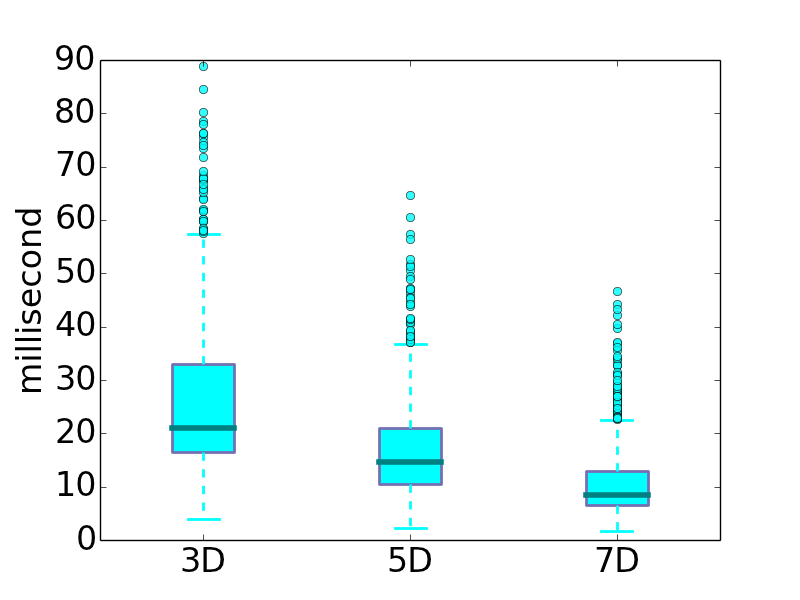
\includegraphics[height=1.5in]{figs/dimenstudy/amg_box}
        \caption{AMG}
        \label{fig:dimen-amg}
    \end{subfigure}%
    \hspace{1em}%
    \begin{subfigure}[t]{0.32\textwidth}
        \centering
        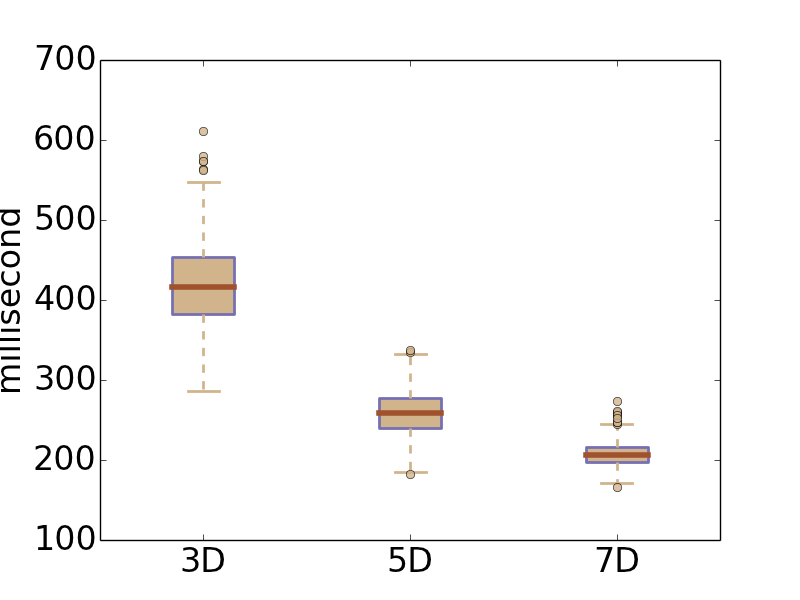
\includegraphics[height=1.5in]{figs/dimenstudy/cr_box}
        \caption{CrystalRouter}
        \label{fig:dimen-cr}
    \end{subfigure}%
    \begin{subfigure}[t]{0.32\textwidth}
        \centering
        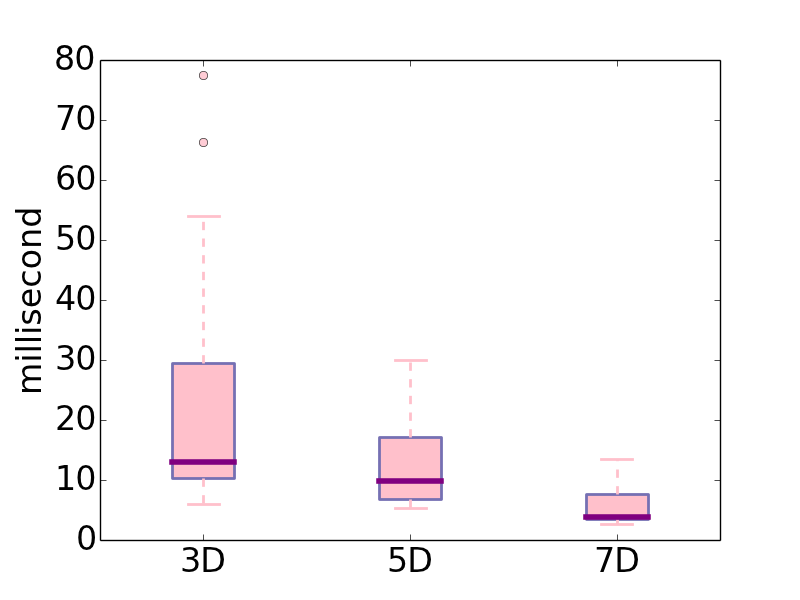
\includegraphics[height=1.5in]{figs/dimenstudy/mg_box}
        \caption{MultiGrid}
        \label{fig:dimen-mg}
    \end{subfigure}%
   \caption{Data Transfer Time of AMG, CrystalRouter and MultiGrid on 3D, 5D and 7D torus network, with constant per-link bandwidth.}
   \label{fig:dimensionality-study}
\end{figure*}

In the fixed link bandwidth experiment, shown in Figure~\ref{fig:dimensionality-study}, the data transfer time of the three applications are significantly reduced as the dimensionality increases, so the applications can easily make use of the increased dimensionality (lower hops on average) and/or aggregate bandwidth (more links being concurrently used). Interestingly, AMG has the greatest degree of outliers compared to the others. We expect this to be a combination of non-optimal rank mappings causing a greater degree of variance due to the highly regular communication pattern and the distribution of message sizes. MultiGrid seems to benefit the most in terms of reducing the spread of the time distribution, though the median message time remains roughly within a factor of two. The time distribution in CrystalRouter seems to accrue the most benefits, likely due to the combination of cross-cutting and localized per-rank traffic.

\begin{figure*}[t!]
    \centering
    \begin{subfigure}[t]{0.32\textwidth}
        \centering
        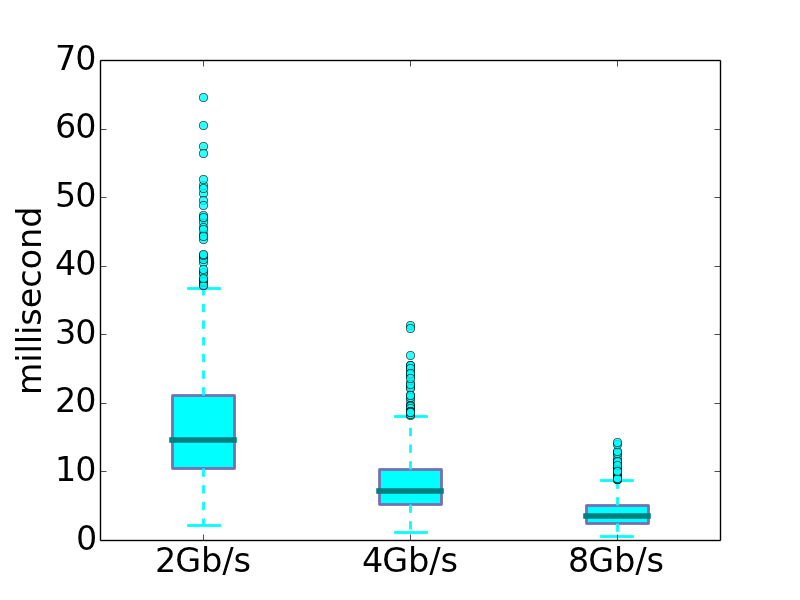
\includegraphics[height=1.5in]{figs/bandwidthstudy/amg_bw_box}
        \caption{AMG}
        \label{fig:bdwstudy-amg}
    \end{subfigure}%
    \hspace{1em}%
    \begin{subfigure}[t]{0.32\textwidth}
        \centering
        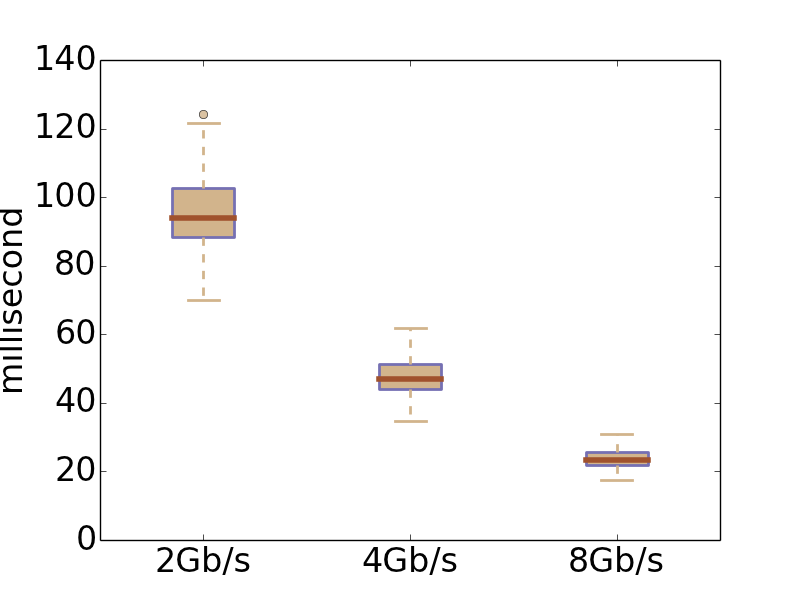
\includegraphics[height=1.5in]{figs/bandwidthstudy/cr_bw_box}
        \caption{CrystalRouter}
        \label{fig:bdwstudy-cr}
    \end{subfigure}%
    \begin{subfigure}[t]{0.32\textwidth}
        \centering
        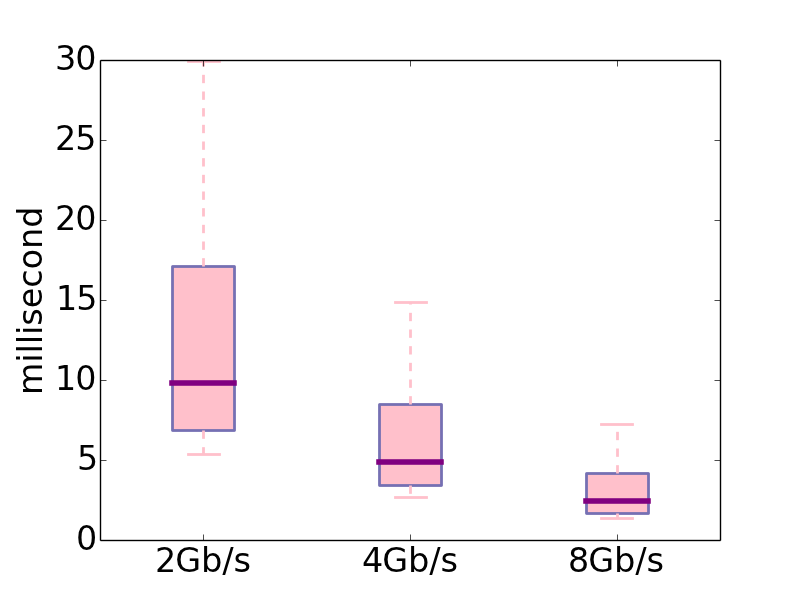
\includegraphics[height=1.5in]{figs/bandwidthstudy/mg_bw_box}
        \caption{MultiGrid}
        \label{fig:bdwstudy-mg}
    \end{subfigure}%
   \caption{Data transfer time of AMG, CrystalRouter and MultiGrid on 5D torus network with 2GiB/s, 4GiB/s and GiB/s direct link bandwidth. }
   \label{fig:bandwidth-study}
\end{figure*}

In the fixed dimensionality experiment, shown in Figure~\ref{fig:bandwidth-study}, the increased per-link bandwidth, expectedly, benefits each application roughly equally, reducing the time distributions linearly.

\begin{figure*}[t!]
    \centering
    \begin{subfigure}[t]{0.32\textwidth}
        \centering
        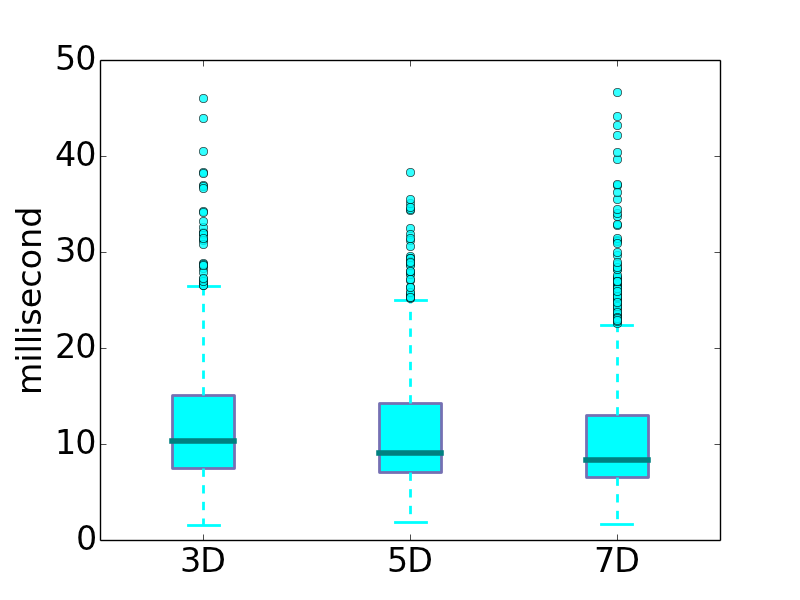
\includegraphics[height=1.5in]{figs/samebdw/amg}
        \caption{AMG}
        \label{fig:samebd-amg}
    \end{subfigure}%
    \hspace{1em}%
    \begin{subfigure}[t]{0.32\textwidth}
        \centering
        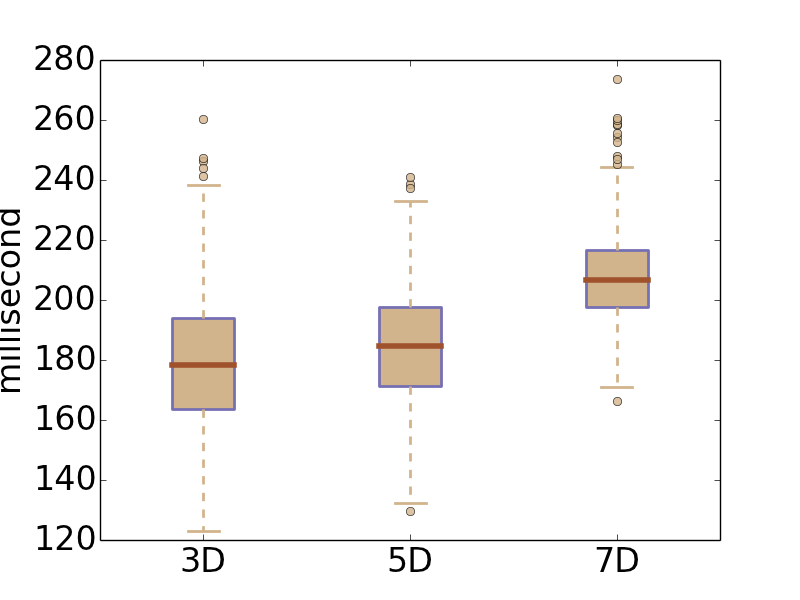
\includegraphics[height=1.5in]{figs/samebdw/cr}
        \caption{CrystalRouter}
        \label{fig:samebd-cr}
    \end{subfigure}%
    \begin{subfigure}[t]{0.32\textwidth}
        \centering
        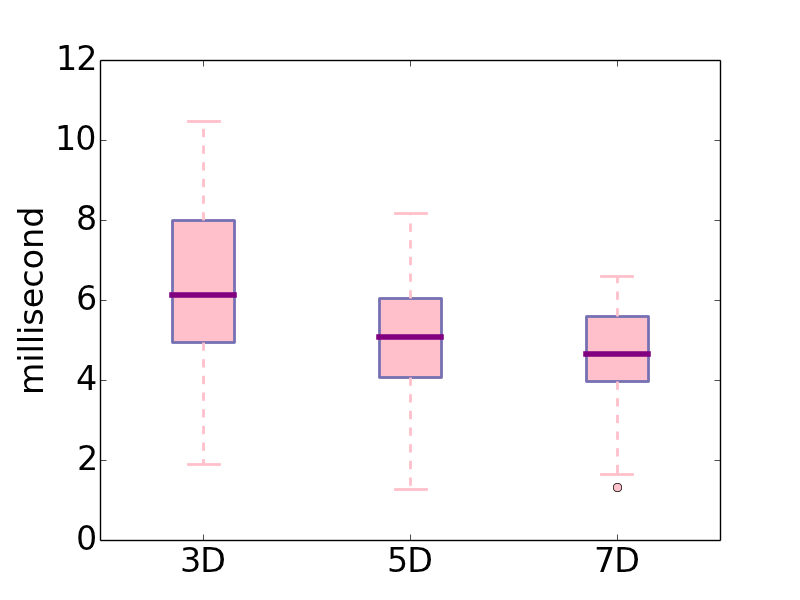
\includegraphics[height=1.5in]{figs/samebdw/mg}
        \caption{MultiGrid}
        \label{fig:samebd-mg}
    \end{subfigure}%
   \caption{Data transfer time of AMG, CrystalRouter and MultiGrid on 3D, 5D and 7D torus network with same aggregated bandwidth. }
   \label{fig: bandwidth-time-box}
\end{figure*}

\begin{table}[ht]
\begin{center}
\caption{Torus networks with same aggregated bandwidth} 
\label{tab: fix-bandwidth}
\begin{tabular}{l c c c} 
\toprule % Top horizontal line
\toprule
&\multicolumn{3}{c}{Bandwidth } \\
\cmidrule(l){2-4}
Dimension  & per-link & aggregate &\\ % Column names row
\midrule % In-table horizontal line
3D      & 4.67GiB/s  & 28GiB/s  & \\  % Content row 1
\midrule % In-table horizontal line
5D    & 2.8GiB/s  & 28GiB/s  &\\ % Content row 1
\midrule % In-table horizontal line
7D    & 2GiB/s & 28GiB/s & \\
\midrule
\bottomrule % Bottom horizontal line
\end{tabular}
\end{center}
\end{table}

In the fixed aggregate bandwidth experiment, with configuration in Table~\ref{tab: fix-bandwidth} and results shown in Figure~\ref{fig: bandwidth-time-box}, the results are more nuanced. At least for these applications, the benefits from increased dimensionality do not outweigh the reduction in per-link bandwidth. MultiGrid does see benefits in the increased dimensionality, particularly with respect to outliers, but has a similar median message time. CrystalRouter reduces performance as the dimensionality increases, but only by a small degree. AMG remains roughly the same, minus a dip in the maximum message time that could be due to rank-to-node mapping changes.



